\subsection{Long-term 2D SLAM in Industrial environments}
In this thesis the focus will be on industrial environments but most of the properties of interest when it comes to mobile robot navigation, localization and mapping holds true for many other types of environments.

\subsubsection{Industrial environment}
In an industrial environment it not uncommon for some areas to be filled with and emptied of obstacles at various speeds. This could for instance be partially completed product awaiting the next part of the manufacturing process or warehouses that could receive large shipments and then be emptied gradually. Due to the variation in any real world scenarios it is necessary to consider the types of objects it is expected to encounter and the goal for each type with respect to the continued mapping.

 
\subsubsection{Characteristics in industrial environments}
\label{sec:characteristics_in_industrial_environments}
An investigation of an representative industrial area where mobile robots are used, shows that areas share common dynamical characteristics. 
During a visit at SCAN A/S a high degree of structure and fixed routines where observed. 
Different work stations produce different parts of the product and place them in areas for the next station to continue on them.
Part of the production line at SCAN A/S, where a MIR robot is used, are shown in figure \ref{fig:scan-mir}. 
The machine is fixed to the floor and is almost as static as the walls in the factory.
Figure \ref{fig:scan-semi-static-obstacles} shows product parts that have been processed by one station, and are ready to be picked up by the next station. 
It might be possible to take advantage of the fixed routines and steady production rate when building and updating a long term map.
As seen in the figure objects are only roughly placed and are not aligned carefully, which can influence mapping with a high resolution grid.

\begin{table}[htbp]
	\caption{Regions of industrial environments}
	\label{tab:regions_of_industrial_environments}
	\begin{center}
		\begin{tabular}{p{2.cm} | p{2.6cm} | p{2.6cm} | p{2.6cm} | p{2.6cm}}
			\toprule
			\textbf{Type} & \textbf{Dominated areas} & \textbf{Object types} & \textbf{In navigation} & \textbf{In localization} \\ 
			\rowcolor[gray]{0.925}
			\textit{Highly dynamic} & Central corridors & Humans, moving vehicles & Avoid these areas if convenient & Consider avoiding this area \\
			\textit{Semi-static} & Temporary Storage areas & Pallets with parts or products & Incorporate for next planning with non-lethal & Landmarks value based on degree of dynamics \\ 
			\rowcolor[gray]{0.925}
			\textit{Static} & The rest & Walls, heavy machinery & Incorporate in map with lethal & Very good landmark \\			
			\bottomrule
		\end{tabular} 
	\end{center}
\end{table}

The areas can roughly be classified based on dynamics of the obstacles that are usually contained within them, as shown in table \ref{tab:regions_of_industrial_environments}. Areas with objects that moves almost constantly like humans are categorized as \textit{highly dynamic}, whereas areas with objects like walls, that never move are categorized as \textit{static}. The remaining \textit{semi-static} objects can be everything from parked vehicles to stored production parts, that moves with minutes or weeks in between. 

\begin{figure}[htbp]
	\centering
	\begin{subfigure}[t]{0.6\textwidth}
		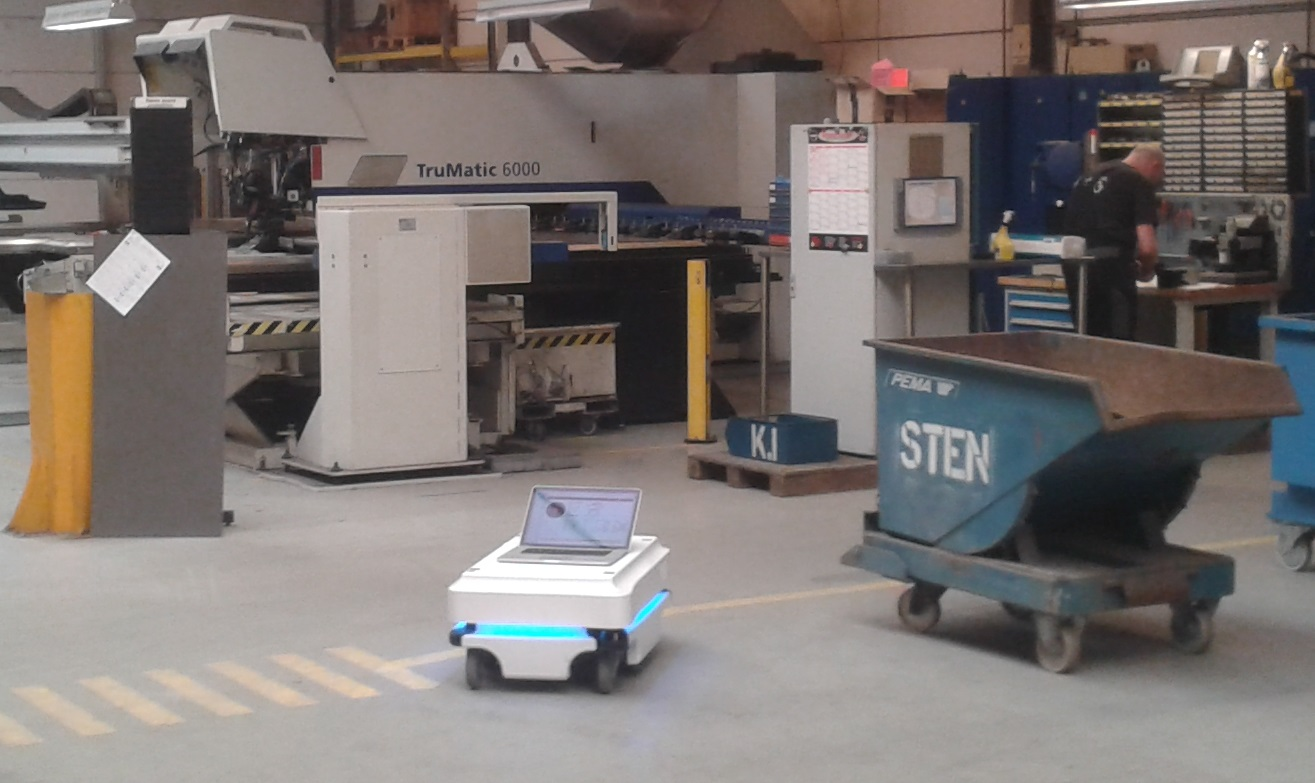
\includegraphics[width=1.0\textwidth]{chapters/mapping_of_dynamic_areas/figures/scan-mir}	
		\caption{MIR 100 robot navigating close to heavy machinery.}
		\label{fig:scan-mir}
	\end{subfigure}
	\begin{subfigure}[t]{0.3875\textwidth}
		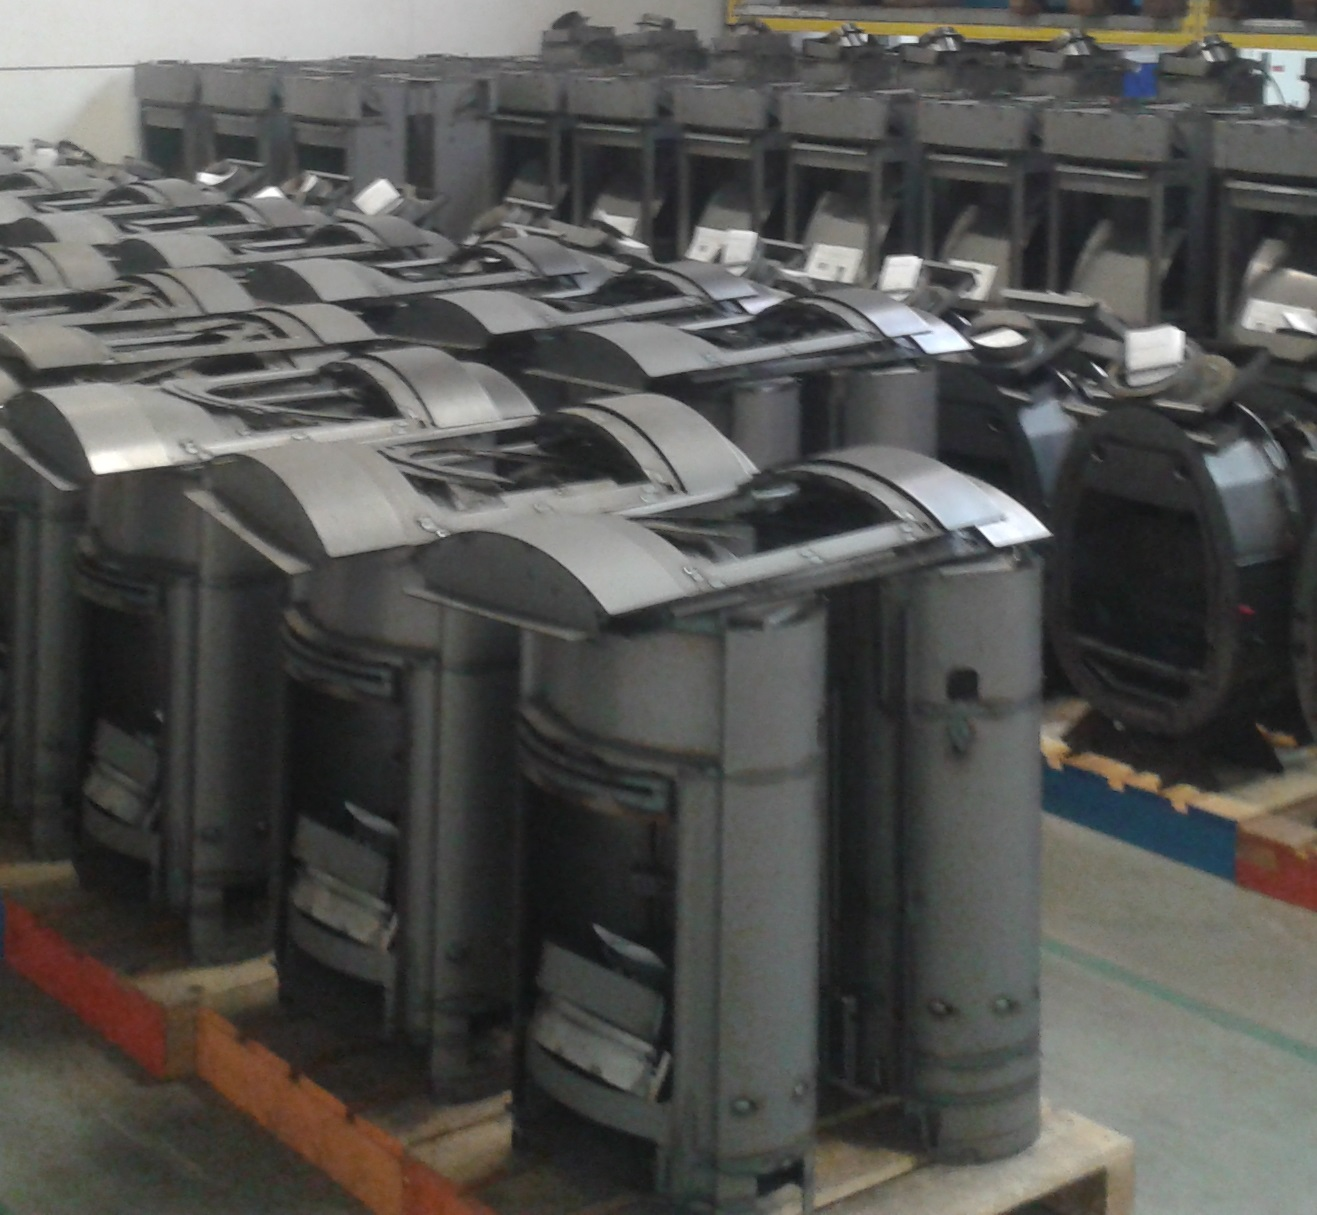
\includegraphics[width=1.0\textwidth]{chapters/mapping_of_dynamic_areas/figures/scan-semi-static-obstacles}
		\caption{\textit{Semi-static} obstacles in the form of product parts.}
		\label{fig:scan-semi-static-obstacles}
	\end{subfigure}
	\caption{Examples of obstacles in the production area at SCAN A/S.}
\end{figure}

The information of these areas can be incorporated in the representation of the world to avoid having to re-plan a path and to improve localization. 

The \textit{highly dynamic} objects should not be considered as obstacles, but some re-planning of the plan might be unavoidable due to them. 
It is beneficial to include \textit{semi-static} obstacles in path planning to avoid having to re-plan, but by assigning them as lethal obstacles it might be impossible to plan a path although one is possible.
The \textit{static} objects should always be present as lethal obstacles when path planning to avoid navigating along obscure routes.

The \textit{highly dynamic} objects should not be included as landmarks for the localization, since they are moving almost constantly. 
Since the value of the \textit{semi-static} obstacles as landmarks depends on how dynamic they are, they should be weighted in the localization algorithm accordingly. 
The \textit{static} obstacles are very good landmarks.

If the \textit{semi-static} obstacles moves at a constant rate, it might be possible to predict the presence of it in the future by learning its transient behavior.
By predicting the presence of obstacles it is possible to plan around them and use them as landmarks, when they are present.
This would be a huge improvements, but during the visit at SCAN A/S it became clear that obstacles are not placed exactly the same place, and the product part travel though the production line.
By steady production pace and fixed areas for product parts, might however introduce similar objects at similar locations and time.

\subsubsection{Observability}
An industrial setup is typical rather large. It is therefore unlikely that a robot will be able to observe the entire operational environment at all times. As changes to the environment are mostly independent of the movement of the robot, this leads to unobserved changes that may cause trouble in learning the dynamics. Depending on the size of the operating area and the frequency of observing a certain area this effect can vary significant throughout the environment.
